% !TeX spellcheck = en_GB
\section{Results}
\label{sec_results}

In the following we present the results from the two scenarios.

\subsection{Dynamic distance}

\begin{figure}		
	
	%\begin{tikzpicture}
%  \begin{axis}
%    [
%	xlabel=meter,
%	ylabel=dBm,
%	xtick={1, 2, 3, 4, 5, 6, 7, 8, 9, 10, 11, 12},
%    xticklabels={0, 2, 4, 6, 8, 10, 12, 14, 16, 18, 20},
%    boxplot/draw direction=y
%    ]
%    
%
%%"00,0"
%\buildBoxPlot{-46}{-45}{-61}{-71}{-44}
%%"00,5"
%%\buildBoxPlot{-57}{-55}{-59}{-61}{-54}
%%"01"
%%\buildBoxPlot{-68}{-67}{-69}{-75}{-65}
%%"02"
%\buildBoxPlot{-69}{-67}{-75}{-85}{-63}
%%"04"
%\buildBoxPlot{-70}{-69}{-71}{-74}{-67}
%%"06"
%\buildBoxPlot{-78}{-76}{-79}{-81}{-72}
%%"08"
%\buildBoxPlot{-78}{-77}{-83}{-90}{-76}
%%"10"
%\buildBoxPlot{-78}{-77}{-80}{-83}{-75}
%%"12"
%\buildBoxPlot{-80}{-77}{-82}{-86}{-75}
%%"14"
%\buildBoxPlot{-77}{-76}{-77}{-78}{-74}
%%"16"
%\buildBoxPlot{-81}{-80}{-82}{-84}{-78}
%%"18"
%\buildBoxPlot{-85}{-83}{-85}{-91}{-81}
%%"20"
%\buildBoxPlot{-84}{-84}{-85}{-88}{-81}
%
%\end{axis}
%	
%\end{tikzpicture}


\begin{tikzpicture}
\begin{axis}
[
xlabel=meter,
ylabel=dBm,
xtick={1, 2, 3, 4, 5, 6, 7, 8, 9, 10, 11, 12, 13, 14},
xticklabels={0.5, 1, 2, 3, 4, 6, 8, 10, 12, 14, 16, 18, 20},
boxplot/draw direction=y
]


%"00.5"                                
\buildBoxPlot{-50}{-46}{-59}{-73}{-43} 
%%"00"                                  
%\buildBoxPlot{-26}{-26}{-27}{-30}{-25} 
%"01"                                  
\buildBoxPlot{-55}{-54}{-58}{-63}{-47} 
%"02"                                  
\buildBoxPlot{-55}{-48}{-58}{-79}{-44} 
%"03"                                  
\buildBoxPlot{-63}{-60}{-66}{-85}{-53} 
%"04"                                  
\buildBoxPlot{-63}{-60}{-68}{-89}{-51} 
%%"05"                                  
%\buildBoxPlot{-68}{-65}{-71}{-84}{-59} 
%"06"                                  
\buildBoxPlot{-69}{-67}{-71}{-90}{-61} 
%%"07"                                  
%\buildBoxPlot{-73}{-68}{-78}{-92}{-63} 
%"08"                                  
%\buildBoxPlot{-73}{-68}{-77}{-90}{-60} 
%%"09"                                  
\buildBoxPlot{-69}{-64}{-71}{-91}{-59} 
%"10"                                  
\buildBoxPlot{-71}{-67}{-75}{-92}{-62} 
%"12"                                  
\buildBoxPlot{-78}{-75}{-82}{-94}{-66} 
%"14"                                  
\buildBoxPlot{-70}{-68}{-73}{-81}{-60} 
%"16"                                  
\buildBoxPlot{-69}{-68}{-77}{-93}{-63} 
%"18"                                  
\buildBoxPlot{-75}{-71}{-78}{-93}{-65} 
%"20"                                  
\buildBoxPlot{-77}{-74}{-80}{-91}{-66} 


\addplot[thick, red] coordinates {
	(1  ,-50)
	(2  ,-55)
	(3  ,-55)
	(4  ,-63)	
	(5  ,-63)	
	(6  ,-69)	
	(7  ,-69)
	(8  ,-71)
	(9  ,-78)
	(10 ,-70)
	(11 ,-69)
	(12 ,-75)
	(13 ,-77)
	
	};
\end{axis}


\end{tikzpicture}

\begin{tikzpicture}
\begin{axis}
[
xlabel=meter,
ylabel=dBm,
xtick={1, 2, 3, 4, 5, 6, 7, 8, 9, 10, 11, 12, 13, 14},
xticklabels={0.5, 1, 2, 3, 4, 6, 8, 10, 12, 14, 16, 18, 20},
boxplot/draw direction=y
]


%%"00"
%\buildBoxPlot{-19}{-18}{-22}{-23}{-18}
%"00.5"
\buildBoxPlot{-43}{-42}{-45}{-49}{-41}
%"01"
\buildBoxPlot{-50}{-48}{-52}{-63}{-44}
%"02"
\buildBoxPlot{-58}{-53}{-62}{-81}{-46}
%"03"
\buildBoxPlot{-61}{-58}{-65}{-86}{-49}
%%"05"
%\buildBoxPlot{-64}{-62}{-66}{-80}{-55}
%"04"
\buildBoxPlot{-63}{-58}{-66}{-85}{-52}
%"06"
%\buildBoxPlot{-62}{-59}{-70}{-78}{-53}
%%"07"
\buildBoxPlot{-65}{-61}{-67}{-83}{-51}
%"08"
%\buildBoxPlot{-70}{-68}{-74}{-89}{-60}
%%"09"
\buildBoxPlot{-73}{-70}{-77}{-92}{-62}
%"12"
\buildBoxPlot{-62}{-61}{-64}{-75}{-57}
%"10"
\buildBoxPlot{-65}{-62}{-70}{-90}{-57}
%"16"
\buildBoxPlot{-63}{-62}{-65}{-71}{-56}
%"20"
\buildBoxPlot{-71}{-71}{-72}{-85}{-67}
%"14"
\buildBoxPlot{-68}{-64}{-71}{-81}{-57}
%"18"
\buildBoxPlot{-75}{-73}{-80}{-91}{-69}


\addplot[thick, red] coordinates {
	(1  ,-43)
	(2  ,-50)
	(3  ,-58)	
	(4  ,-61)	
	(5  ,-63)	
	(6  ,-65)
	(7  ,-73)
	(8  ,-62)
	(9 ,-65)
	(10 ,-63)
	(11 ,-71)
	(12 ,-68)
	(13 ,-75)
		
};

\end{axis}

\end{tikzpicture}

	
	\caption{ Dynamic distance measurements }
	\label{graf_DynamicMesurements}
	
\end{figure}

The data from this scenario is presented in \cref{graf_DynamicMesurements}.

Seeing how the value of the RSSI measured from the device fluctuates it is clear that RSSI is hard to use for distance measurements.
From a mean around 45 when measured right on top of the system the RSSI value drops drastically within the first few meters.
As the device moves further away from the system the RSSI value becomes lower but there is no apparent model to the decline.

The noise seams to fluctuate more towards the noise side of the mean. This suggests that if a lower value is measured it is more reliable then a high value, witch fits in well for authentication purposes.
Since most outliers are in the lower dBm end, there is a greater chance that you will be incorrectly logged out as a result of noise than incorrectly logged in.


\subsection{Static distance}
\begin{figure}
	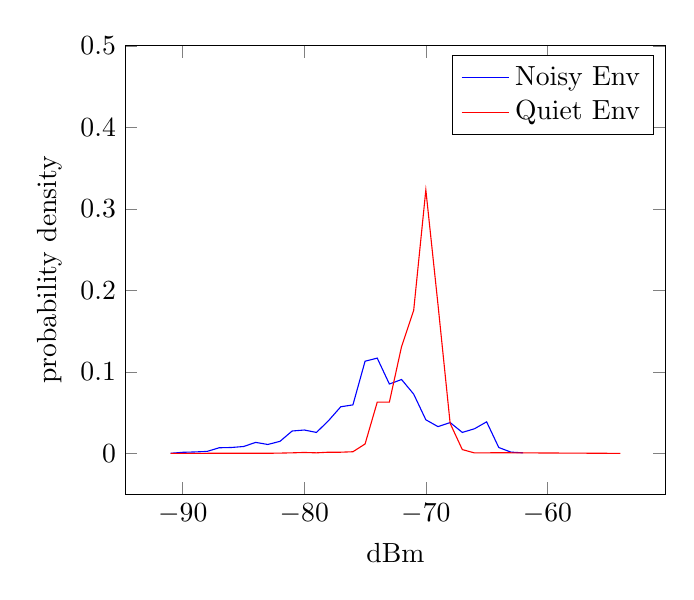
\begin{tikzpicture}
\begin{axis}[ymax=0.5,xlabel=dBm,ylabel=probability density]
\addplot[blue!20!blue] coordinates {
	(-91 ,0.0001093255)
	(-90 ,0.0013119055)
	(-89 ,0.0017492074)
	(-88 ,0.0024051602)
	(-87 ,0.0068875041)
	(-86 ,0.0072154805)
	(-85 ,0.0084180606)
	(-84 ,0.0134470318)
	(-83 ,0.0109325462)
	(-82 ,0.0147589374)
	(-81 ,0.0274406909)
	(-80 ,0.028643271)
	(-79 ,0.0256914835)
	(-78 ,0.04023177)
	(-77 ,0.0571772166)
	(-76 ,0.0594730513)
	(-75 ,0.1130425276)
	(-74 ,0.1168689188)
	(-73 ,0.0850552094)
	(-72 ,0.0906308079)
	(-71 ,0.0727014322)
	(-70 ,0.0412156991)
	(-69 ,0.0327976386)
	(-68 ,0.0378266098)
	(-67 ,0.0256914835)
	(-66 ,0.0301738275)
	(-65 ,0.0387012135)
	(-64 ,0.0072154805)
	(-63 ,0.0015305565)
	(-62 ,0.0006559528)

		};
\addplot[red!20!red] coordinates {
	(-91, 0)
	(-87, 0.0001107297)
	(-86, 0.0001107297)
	(-83, 0.0001107297)
	(-82, 0.0003321891)
	(-81, 0.0006643783)
	(-80, 0.0011072971)
	(-79, 0.0006643783)
	(-78, 0.0014394862)
	(-77, 0.0014394862)
	(-76, 0.0019931348)
	(-75, 0.0115158897)
	(-74, 0.0627837449)
	(-73, 0.0628944746)
	(-72, 0.1308825158)
	(-71, 0.1755065884)
	(-70, 0.3232200199)
	(-69, 0.1824825601)
	(-68, 0.0367622633)
	(-67, 0.0046506478)
	(-66, 0.0005536485)
	(-64, 0.000775108)
	(-54, 0)
	};
\legend{Noisy Env,Quiet Env}
\end{axis}
\end{tikzpicture}

	
	\caption{Static distance measurements}
	\label{graf_StaticMesurements}
\end{figure}

The results from this experiment clearly shows that the RSSI value becomes less reliable the more noise there is in the environment.
The Noise level will affect how the hysteresis thresholds should be configured.
With too much noise in the environment the mean value of the graph will become indistinctable form the rest.
The data from this scenario is presented in \cref{graf_StaticMesurements}. 



